\documentclass[tikz,border=7pt]{standalone}
\usepackage{amsmath}
\usetikzlibrary{arrows.meta,positioning,calc}

\tikzset{
  comp/.style={draw,rectangle,minimum width=25mm,minimum height=12mm,align=center},
  sum/.style={draw,circle,minimum size=7mm,inner sep=0pt},
  signal/.style={-{Latex[length=2.2mm]},thick}
}

\begin{document}
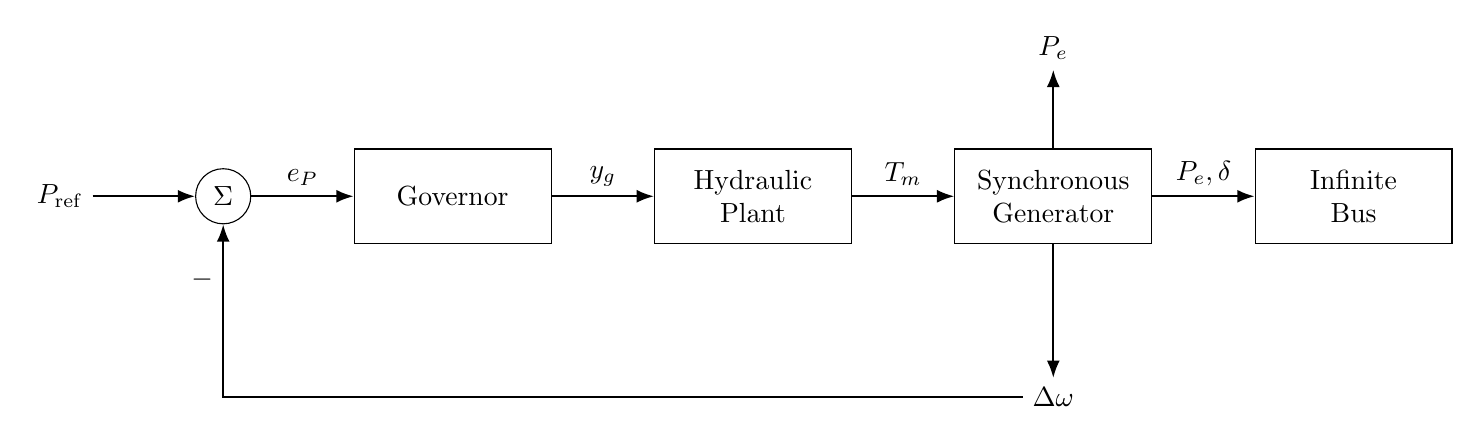
\begin{tikzpicture}[node distance=12mm and 13mm]

\node (pref) {$P_{\mathrm{ref}}$};
\node[sum,right=of pref] (sum) {$\Sigma$};
\node[comp,right=of sum] (gov) {Governor};
\node[comp,right=of gov] (hydro) {Hydraulic\\Plant};
\node[comp,right=of hydro] (gen) {Synchronous\\Generator};
\node[comp,right=of gen] (grid) {Infinite\\Bus};

\node[below=17mm of gen] (freq) {$\Delta \omega$};
\node[above=10mm of gen] (pe) {$P_e$};

\draw[signal] (pref) -- (sum);
\draw[signal] (sum) -- node[above] {$e_P$} (gov);
\draw[signal] (gov) -- node[above] {$y_g$} (hydro);
\draw[signal] (hydro) -- node[above] {$T_m$} (gen);
\draw[signal] (gen) -- node[above] {$P_e,\delta$} (grid);
\draw[signal] (gen.north) -- (pe);
\draw[signal] (gen.south) -- (freq);
\draw[signal] (freq) -| node[pos=0.84,left] {$-$} (sum.south);

\end{tikzpicture}
\end{document}
